\documentclass[11pt]{article}

    \usepackage[breakable]{tcolorbox}
    \usepackage{parskip} % Stop auto-indenting (to mimic markdown behaviour)
    

    % Basic figure setup, for now with no caption control since it's done
    % automatically by Pandoc (which extracts ![](path) syntax from Markdown).
    \usepackage{graphicx}
    % Keep aspect ratio if custom image width or height is specified
    \setkeys{Gin}{keepaspectratio}
    % Maintain compatibility with old templates. Remove in nbconvert 6.0
    \let\Oldincludegraphics\includegraphics
    % Ensure that by default, figures have no caption (until we provide a
    % proper Figure object with a Caption API and a way to capture that
    % in the conversion process - todo).
    \usepackage{caption}
    \DeclareCaptionFormat{nocaption}{}
    \captionsetup{format=nocaption,aboveskip=0pt,belowskip=0pt}

    \usepackage{float}
    \floatplacement{figure}{H} % forces figures to be placed at the correct location
    \usepackage{xcolor} % Allow colors to be defined
    \usepackage{enumerate} % Needed for markdown enumerations to work
    \usepackage{geometry} % Used to adjust the document margins
    \usepackage{amsmath} % Equations
    \usepackage{amssymb} % Equations
    \usepackage{textcomp} % defines textquotesingle
    % Hack from http://tex.stackexchange.com/a/47451/13684:
    \AtBeginDocument{%
        \def\PYZsq{\textquotesingle}% Upright quotes in Pygmentized code
    }
    \usepackage{upquote} % Upright quotes for verbatim code
    \usepackage{eurosym} % defines \euro

    \usepackage{iftex}
    \ifPDFTeX
        \usepackage[T1]{fontenc}
        \IfFileExists{alphabeta.sty}{
              \usepackage{alphabeta}
          }{
              \usepackage[mathletters]{ucs}
              \usepackage[utf8x]{inputenc}
          }
    \else
        \usepackage{fontspec}
        \usepackage{unicode-math}
    \fi

    \usepackage{fancyvrb} % verbatim replacement that allows latex
    \usepackage{grffile} % extends the file name processing of package graphics
                         % to support a larger range
    \makeatletter % fix for old versions of grffile with XeLaTeX
    \@ifpackagelater{grffile}{2019/11/01}
    {
      % Do nothing on new versions
    }
    {
      \def\Gread@@xetex#1{%
        \IfFileExists{"\Gin@base".bb}%
        {\Gread@eps{\Gin@base.bb}}%
        {\Gread@@xetex@aux#1}%
      }
    }
    \makeatother
    \usepackage[Export]{adjustbox} % Used to constrain images to a maximum size
    \adjustboxset{max size={0.9\linewidth}{0.9\paperheight}}

    % The hyperref package gives us a pdf with properly built
    % internal navigation ('pdf bookmarks' for the table of contents,
    % internal cross-reference links, web links for URLs, etc.)
    \usepackage{hyperref}
    % The default LaTeX title has an obnoxious amount of whitespace. By default,
    % titling removes some of it. It also provides customization options.
    \usepackage{titling}
    \usepackage{longtable} % longtable support required by pandoc >1.10
    \usepackage{booktabs}  % table support for pandoc > 1.12.2
    \usepackage{array}     % table support for pandoc >= 2.11.3
    \usepackage{calc}      % table minipage width calculation for pandoc >= 2.11.1
    \usepackage[inline]{enumitem} % IRkernel/repr support (it uses the enumerate* environment)
    \usepackage[normalem]{ulem} % ulem is needed to support strikethroughs (\sout)
                                % normalem makes italics be italics, not underlines
    \usepackage{soul}      % strikethrough (\st) support for pandoc >= 3.0.0
    \usepackage{mathrsfs}
    

    
    % Colors for the hyperref package
    \definecolor{urlcolor}{rgb}{0,.145,.698}
    \definecolor{linkcolor}{rgb}{.71,0.21,0.01}
    \definecolor{citecolor}{rgb}{.12,.54,.11}

    % ANSI colors
    \definecolor{ansi-black}{HTML}{3E424D}
    \definecolor{ansi-black-intense}{HTML}{282C36}
    \definecolor{ansi-red}{HTML}{E75C58}
    \definecolor{ansi-red-intense}{HTML}{B22B31}
    \definecolor{ansi-green}{HTML}{00A250}
    \definecolor{ansi-green-intense}{HTML}{007427}
    \definecolor{ansi-yellow}{HTML}{DDB62B}
    \definecolor{ansi-yellow-intense}{HTML}{B27D12}
    \definecolor{ansi-blue}{HTML}{208FFB}
    \definecolor{ansi-blue-intense}{HTML}{0065CA}
    \definecolor{ansi-magenta}{HTML}{D160C4}
    \definecolor{ansi-magenta-intense}{HTML}{A03196}
    \definecolor{ansi-cyan}{HTML}{60C6C8}
    \definecolor{ansi-cyan-intense}{HTML}{258F8F}
    \definecolor{ansi-white}{HTML}{C5C1B4}
    \definecolor{ansi-white-intense}{HTML}{A1A6B2}
    \definecolor{ansi-default-inverse-fg}{HTML}{FFFFFF}
    \definecolor{ansi-default-inverse-bg}{HTML}{000000}

    % common color for the border for error outputs.
    \definecolor{outerrorbackground}{HTML}{FFDFDF}

    % commands and environments needed by pandoc snippets
    % extracted from the output of `pandoc -s`
    \providecommand{\tightlist}{%
      \setlength{\itemsep}{0pt}\setlength{\parskip}{0pt}}
    \DefineVerbatimEnvironment{Highlighting}{Verbatim}{commandchars=\\\{\}}
    % Add ',fontsize=\small' for more characters per line
    \newenvironment{Shaded}{}{}
    \newcommand{\KeywordTok}[1]{\textcolor[rgb]{0.00,0.44,0.13}{\textbf{{#1}}}}
    \newcommand{\DataTypeTok}[1]{\textcolor[rgb]{0.56,0.13,0.00}{{#1}}}
    \newcommand{\DecValTok}[1]{\textcolor[rgb]{0.25,0.63,0.44}{{#1}}}
    \newcommand{\BaseNTok}[1]{\textcolor[rgb]{0.25,0.63,0.44}{{#1}}}
    \newcommand{\FloatTok}[1]{\textcolor[rgb]{0.25,0.63,0.44}{{#1}}}
    \newcommand{\CharTok}[1]{\textcolor[rgb]{0.25,0.44,0.63}{{#1}}}
    \newcommand{\StringTok}[1]{\textcolor[rgb]{0.25,0.44,0.63}{{#1}}}
    \newcommand{\CommentTok}[1]{\textcolor[rgb]{0.38,0.63,0.69}{\textit{{#1}}}}
    \newcommand{\OtherTok}[1]{\textcolor[rgb]{0.00,0.44,0.13}{{#1}}}
    \newcommand{\AlertTok}[1]{\textcolor[rgb]{1.00,0.00,0.00}{\textbf{{#1}}}}
    \newcommand{\FunctionTok}[1]{\textcolor[rgb]{0.02,0.16,0.49}{{#1}}}
    \newcommand{\RegionMarkerTok}[1]{{#1}}
    \newcommand{\ErrorTok}[1]{\textcolor[rgb]{1.00,0.00,0.00}{\textbf{{#1}}}}
    \newcommand{\NormalTok}[1]{{#1}}

    % Additional commands for more recent versions of Pandoc
    \newcommand{\ConstantTok}[1]{\textcolor[rgb]{0.53,0.00,0.00}{{#1}}}
    \newcommand{\SpecialCharTok}[1]{\textcolor[rgb]{0.25,0.44,0.63}{{#1}}}
    \newcommand{\VerbatimStringTok}[1]{\textcolor[rgb]{0.25,0.44,0.63}{{#1}}}
    \newcommand{\SpecialStringTok}[1]{\textcolor[rgb]{0.73,0.40,0.53}{{#1}}}
    \newcommand{\ImportTok}[1]{{#1}}
    \newcommand{\DocumentationTok}[1]{\textcolor[rgb]{0.73,0.13,0.13}{\textit{{#1}}}}
    \newcommand{\AnnotationTok}[1]{\textcolor[rgb]{0.38,0.63,0.69}{\textbf{\textit{{#1}}}}}
    \newcommand{\CommentVarTok}[1]{\textcolor[rgb]{0.38,0.63,0.69}{\textbf{\textit{{#1}}}}}
    \newcommand{\VariableTok}[1]{\textcolor[rgb]{0.10,0.09,0.49}{{#1}}}
    \newcommand{\ControlFlowTok}[1]{\textcolor[rgb]{0.00,0.44,0.13}{\textbf{{#1}}}}
    \newcommand{\OperatorTok}[1]{\textcolor[rgb]{0.40,0.40,0.40}{{#1}}}
    \newcommand{\BuiltInTok}[1]{{#1}}
    \newcommand{\ExtensionTok}[1]{{#1}}
    \newcommand{\PreprocessorTok}[1]{\textcolor[rgb]{0.74,0.48,0.00}{{#1}}}
    \newcommand{\AttributeTok}[1]{\textcolor[rgb]{0.49,0.56,0.16}{{#1}}}
    \newcommand{\InformationTok}[1]{\textcolor[rgb]{0.38,0.63,0.69}{\textbf{\textit{{#1}}}}}
    \newcommand{\WarningTok}[1]{\textcolor[rgb]{0.38,0.63,0.69}{\textbf{\textit{{#1}}}}}


    % Define a nice break command that doesn't care if a line doesn't already
    % exist.
    \def\br{\hspace*{\fill} \\* }
    % Math Jax compatibility definitions
    \def\gt{>}
    \def\lt{<}
    \let\Oldtex\TeX
    \let\Oldlatex\LaTeX
    \renewcommand{\TeX}{\textrm{\Oldtex}}
    \renewcommand{\LaTeX}{\textrm{\Oldlatex}}
    % Document parameters
    % Document title
    \title{REPORT}
    
    
    
    
    
    
    
% Pygments definitions
\makeatletter
\def\PY@reset{\let\PY@it=\relax \let\PY@bf=\relax%
    \let\PY@ul=\relax \let\PY@tc=\relax%
    \let\PY@bc=\relax \let\PY@ff=\relax}
\def\PY@tok#1{\csname PY@tok@#1\endcsname}
\def\PY@toks#1+{\ifx\relax#1\empty\else%
    \PY@tok{#1}\expandafter\PY@toks\fi}
\def\PY@do#1{\PY@bc{\PY@tc{\PY@ul{%
    \PY@it{\PY@bf{\PY@ff{#1}}}}}}}
\def\PY#1#2{\PY@reset\PY@toks#1+\relax+\PY@do{#2}}

\@namedef{PY@tok@w}{\def\PY@tc##1{\textcolor[rgb]{0.73,0.73,0.73}{##1}}}
\@namedef{PY@tok@c}{\let\PY@it=\textit\def\PY@tc##1{\textcolor[rgb]{0.24,0.48,0.48}{##1}}}
\@namedef{PY@tok@cp}{\def\PY@tc##1{\textcolor[rgb]{0.61,0.40,0.00}{##1}}}
\@namedef{PY@tok@k}{\let\PY@bf=\textbf\def\PY@tc##1{\textcolor[rgb]{0.00,0.50,0.00}{##1}}}
\@namedef{PY@tok@kp}{\def\PY@tc##1{\textcolor[rgb]{0.00,0.50,0.00}{##1}}}
\@namedef{PY@tok@kt}{\def\PY@tc##1{\textcolor[rgb]{0.69,0.00,0.25}{##1}}}
\@namedef{PY@tok@o}{\def\PY@tc##1{\textcolor[rgb]{0.40,0.40,0.40}{##1}}}
\@namedef{PY@tok@ow}{\let\PY@bf=\textbf\def\PY@tc##1{\textcolor[rgb]{0.67,0.13,1.00}{##1}}}
\@namedef{PY@tok@nb}{\def\PY@tc##1{\textcolor[rgb]{0.00,0.50,0.00}{##1}}}
\@namedef{PY@tok@nf}{\def\PY@tc##1{\textcolor[rgb]{0.00,0.00,1.00}{##1}}}
\@namedef{PY@tok@nc}{\let\PY@bf=\textbf\def\PY@tc##1{\textcolor[rgb]{0.00,0.00,1.00}{##1}}}
\@namedef{PY@tok@nn}{\let\PY@bf=\textbf\def\PY@tc##1{\textcolor[rgb]{0.00,0.00,1.00}{##1}}}
\@namedef{PY@tok@ne}{\let\PY@bf=\textbf\def\PY@tc##1{\textcolor[rgb]{0.80,0.25,0.22}{##1}}}
\@namedef{PY@tok@nv}{\def\PY@tc##1{\textcolor[rgb]{0.10,0.09,0.49}{##1}}}
\@namedef{PY@tok@no}{\def\PY@tc##1{\textcolor[rgb]{0.53,0.00,0.00}{##1}}}
\@namedef{PY@tok@nl}{\def\PY@tc##1{\textcolor[rgb]{0.46,0.46,0.00}{##1}}}
\@namedef{PY@tok@ni}{\let\PY@bf=\textbf\def\PY@tc##1{\textcolor[rgb]{0.44,0.44,0.44}{##1}}}
\@namedef{PY@tok@na}{\def\PY@tc##1{\textcolor[rgb]{0.41,0.47,0.13}{##1}}}
\@namedef{PY@tok@nt}{\let\PY@bf=\textbf\def\PY@tc##1{\textcolor[rgb]{0.00,0.50,0.00}{##1}}}
\@namedef{PY@tok@nd}{\def\PY@tc##1{\textcolor[rgb]{0.67,0.13,1.00}{##1}}}
\@namedef{PY@tok@s}{\def\PY@tc##1{\textcolor[rgb]{0.73,0.13,0.13}{##1}}}
\@namedef{PY@tok@sd}{\let\PY@it=\textit\def\PY@tc##1{\textcolor[rgb]{0.73,0.13,0.13}{##1}}}
\@namedef{PY@tok@si}{\let\PY@bf=\textbf\def\PY@tc##1{\textcolor[rgb]{0.64,0.35,0.47}{##1}}}
\@namedef{PY@tok@se}{\let\PY@bf=\textbf\def\PY@tc##1{\textcolor[rgb]{0.67,0.36,0.12}{##1}}}
\@namedef{PY@tok@sr}{\def\PY@tc##1{\textcolor[rgb]{0.64,0.35,0.47}{##1}}}
\@namedef{PY@tok@ss}{\def\PY@tc##1{\textcolor[rgb]{0.10,0.09,0.49}{##1}}}
\@namedef{PY@tok@sx}{\def\PY@tc##1{\textcolor[rgb]{0.00,0.50,0.00}{##1}}}
\@namedef{PY@tok@m}{\def\PY@tc##1{\textcolor[rgb]{0.40,0.40,0.40}{##1}}}
\@namedef{PY@tok@gh}{\let\PY@bf=\textbf\def\PY@tc##1{\textcolor[rgb]{0.00,0.00,0.50}{##1}}}
\@namedef{PY@tok@gu}{\let\PY@bf=\textbf\def\PY@tc##1{\textcolor[rgb]{0.50,0.00,0.50}{##1}}}
\@namedef{PY@tok@gd}{\def\PY@tc##1{\textcolor[rgb]{0.63,0.00,0.00}{##1}}}
\@namedef{PY@tok@gi}{\def\PY@tc##1{\textcolor[rgb]{0.00,0.52,0.00}{##1}}}
\@namedef{PY@tok@gr}{\def\PY@tc##1{\textcolor[rgb]{0.89,0.00,0.00}{##1}}}
\@namedef{PY@tok@ge}{\let\PY@it=\textit}
\@namedef{PY@tok@gs}{\let\PY@bf=\textbf}
\@namedef{PY@tok@ges}{\let\PY@bf=\textbf\let\PY@it=\textit}
\@namedef{PY@tok@gp}{\let\PY@bf=\textbf\def\PY@tc##1{\textcolor[rgb]{0.00,0.00,0.50}{##1}}}
\@namedef{PY@tok@go}{\def\PY@tc##1{\textcolor[rgb]{0.44,0.44,0.44}{##1}}}
\@namedef{PY@tok@gt}{\def\PY@tc##1{\textcolor[rgb]{0.00,0.27,0.87}{##1}}}
\@namedef{PY@tok@err}{\def\PY@bc##1{{\setlength{\fboxsep}{\string -\fboxrule}\fcolorbox[rgb]{1.00,0.00,0.00}{1,1,1}{\strut ##1}}}}
\@namedef{PY@tok@kc}{\let\PY@bf=\textbf\def\PY@tc##1{\textcolor[rgb]{0.00,0.50,0.00}{##1}}}
\@namedef{PY@tok@kd}{\let\PY@bf=\textbf\def\PY@tc##1{\textcolor[rgb]{0.00,0.50,0.00}{##1}}}
\@namedef{PY@tok@kn}{\let\PY@bf=\textbf\def\PY@tc##1{\textcolor[rgb]{0.00,0.50,0.00}{##1}}}
\@namedef{PY@tok@kr}{\let\PY@bf=\textbf\def\PY@tc##1{\textcolor[rgb]{0.00,0.50,0.00}{##1}}}
\@namedef{PY@tok@bp}{\def\PY@tc##1{\textcolor[rgb]{0.00,0.50,0.00}{##1}}}
\@namedef{PY@tok@fm}{\def\PY@tc##1{\textcolor[rgb]{0.00,0.00,1.00}{##1}}}
\@namedef{PY@tok@vc}{\def\PY@tc##1{\textcolor[rgb]{0.10,0.09,0.49}{##1}}}
\@namedef{PY@tok@vg}{\def\PY@tc##1{\textcolor[rgb]{0.10,0.09,0.49}{##1}}}
\@namedef{PY@tok@vi}{\def\PY@tc##1{\textcolor[rgb]{0.10,0.09,0.49}{##1}}}
\@namedef{PY@tok@vm}{\def\PY@tc##1{\textcolor[rgb]{0.10,0.09,0.49}{##1}}}
\@namedef{PY@tok@sa}{\def\PY@tc##1{\textcolor[rgb]{0.73,0.13,0.13}{##1}}}
\@namedef{PY@tok@sb}{\def\PY@tc##1{\textcolor[rgb]{0.73,0.13,0.13}{##1}}}
\@namedef{PY@tok@sc}{\def\PY@tc##1{\textcolor[rgb]{0.73,0.13,0.13}{##1}}}
\@namedef{PY@tok@dl}{\def\PY@tc##1{\textcolor[rgb]{0.73,0.13,0.13}{##1}}}
\@namedef{PY@tok@s2}{\def\PY@tc##1{\textcolor[rgb]{0.73,0.13,0.13}{##1}}}
\@namedef{PY@tok@sh}{\def\PY@tc##1{\textcolor[rgb]{0.73,0.13,0.13}{##1}}}
\@namedef{PY@tok@s1}{\def\PY@tc##1{\textcolor[rgb]{0.73,0.13,0.13}{##1}}}
\@namedef{PY@tok@mb}{\def\PY@tc##1{\textcolor[rgb]{0.40,0.40,0.40}{##1}}}
\@namedef{PY@tok@mf}{\def\PY@tc##1{\textcolor[rgb]{0.40,0.40,0.40}{##1}}}
\@namedef{PY@tok@mh}{\def\PY@tc##1{\textcolor[rgb]{0.40,0.40,0.40}{##1}}}
\@namedef{PY@tok@mi}{\def\PY@tc##1{\textcolor[rgb]{0.40,0.40,0.40}{##1}}}
\@namedef{PY@tok@il}{\def\PY@tc##1{\textcolor[rgb]{0.40,0.40,0.40}{##1}}}
\@namedef{PY@tok@mo}{\def\PY@tc##1{\textcolor[rgb]{0.40,0.40,0.40}{##1}}}
\@namedef{PY@tok@ch}{\let\PY@it=\textit\def\PY@tc##1{\textcolor[rgb]{0.24,0.48,0.48}{##1}}}
\@namedef{PY@tok@cm}{\let\PY@it=\textit\def\PY@tc##1{\textcolor[rgb]{0.24,0.48,0.48}{##1}}}
\@namedef{PY@tok@cpf}{\let\PY@it=\textit\def\PY@tc##1{\textcolor[rgb]{0.24,0.48,0.48}{##1}}}
\@namedef{PY@tok@c1}{\let\PY@it=\textit\def\PY@tc##1{\textcolor[rgb]{0.24,0.48,0.48}{##1}}}
\@namedef{PY@tok@cs}{\let\PY@it=\textit\def\PY@tc##1{\textcolor[rgb]{0.24,0.48,0.48}{##1}}}

\def\PYZbs{\char`\\}
\def\PYZus{\char`\_}
\def\PYZob{\char`\{}
\def\PYZcb{\char`\}}
\def\PYZca{\char`\^}
\def\PYZam{\char`\&}
\def\PYZlt{\char`\<}
\def\PYZgt{\char`\>}
\def\PYZsh{\char`\#}
\def\PYZpc{\char`\%}
\def\PYZdl{\char`\$}
\def\PYZhy{\char`\-}
\def\PYZsq{\char`\'}
\def\PYZdq{\char`\"}
\def\PYZti{\char`\~}
% for compatibility with earlier versions
\def\PYZat{@}
\def\PYZlb{[}
\def\PYZrb{]}
\makeatother


    % For linebreaks inside Verbatim environment from package fancyvrb.
    \makeatletter
        \newbox\Wrappedcontinuationbox
        \newbox\Wrappedvisiblespacebox
        \newcommand*\Wrappedvisiblespace {\textcolor{red}{\textvisiblespace}}
        \newcommand*\Wrappedcontinuationsymbol {\textcolor{red}{\llap{\tiny$\m@th\hookrightarrow$}}}
        \newcommand*\Wrappedcontinuationindent {3ex }
        \newcommand*\Wrappedafterbreak {\kern\Wrappedcontinuationindent\copy\Wrappedcontinuationbox}
        % Take advantage of the already applied Pygments mark-up to insert
        % potential linebreaks for TeX processing.
        %        {, <, #, %, $, ' and ": go to next line.
        %        _, }, ^, &, >, - and ~: stay at end of broken line.
        % Use of \textquotesingle for straight quote.
        \newcommand*\Wrappedbreaksatspecials {%
            \def\PYGZus{\discretionary{\char`\_}{\Wrappedafterbreak}{\char`\_}}%
            \def\PYGZob{\discretionary{}{\Wrappedafterbreak\char`\{}{\char`\{}}%
            \def\PYGZcb{\discretionary{\char`\}}{\Wrappedafterbreak}{\char`\}}}%
            \def\PYGZca{\discretionary{\char`\^}{\Wrappedafterbreak}{\char`\^}}%
            \def\PYGZam{\discretionary{\char`\&}{\Wrappedafterbreak}{\char`\&}}%
            \def\PYGZlt{\discretionary{}{\Wrappedafterbreak\char`\<}{\char`\<}}%
            \def\PYGZgt{\discretionary{\char`\>}{\Wrappedafterbreak}{\char`\>}}%
            \def\PYGZsh{\discretionary{}{\Wrappedafterbreak\char`\#}{\char`\#}}%
            \def\PYGZpc{\discretionary{}{\Wrappedafterbreak\char`\%}{\char`\%}}%
            \def\PYGZdl{\discretionary{}{\Wrappedafterbreak\char`\$}{\char`\$}}%
            \def\PYGZhy{\discretionary{\char`\-}{\Wrappedafterbreak}{\char`\-}}%
            \def\PYGZsq{\discretionary{}{\Wrappedafterbreak\textquotesingle}{\textquotesingle}}%
            \def\PYGZdq{\discretionary{}{\Wrappedafterbreak\char`\"}{\char`\"}}%
            \def\PYGZti{\discretionary{\char`\~}{\Wrappedafterbreak}{\char`\~}}%
        }
        % Some characters . , ; ? ! / are not pygmentized.
        % This macro makes them "active" and they will insert potential linebreaks
        \newcommand*\Wrappedbreaksatpunct {%
            \lccode`\~`\.\lowercase{\def~}{\discretionary{\hbox{\char`\.}}{\Wrappedafterbreak}{\hbox{\char`\.}}}%
            \lccode`\~`\,\lowercase{\def~}{\discretionary{\hbox{\char`\,}}{\Wrappedafterbreak}{\hbox{\char`\,}}}%
            \lccode`\~`\;\lowercase{\def~}{\discretionary{\hbox{\char`\;}}{\Wrappedafterbreak}{\hbox{\char`\;}}}%
            \lccode`\~`\:\lowercase{\def~}{\discretionary{\hbox{\char`\:}}{\Wrappedafterbreak}{\hbox{\char`\:}}}%
            \lccode`\~`\?\lowercase{\def~}{\discretionary{\hbox{\char`\?}}{\Wrappedafterbreak}{\hbox{\char`\?}}}%
            \lccode`\~`\!\lowercase{\def~}{\discretionary{\hbox{\char`\!}}{\Wrappedafterbreak}{\hbox{\char`\!}}}%
            \lccode`\~`\/\lowercase{\def~}{\discretionary{\hbox{\char`\/}}{\Wrappedafterbreak}{\hbox{\char`\/}}}%
            \catcode`\.\active
            \catcode`\,\active
            \catcode`\;\active
            \catcode`\:\active
            \catcode`\?\active
            \catcode`\!\active
            \catcode`\/\active
            \lccode`\~`\~
        }
    \makeatother

    \let\OriginalVerbatim=\Verbatim
    \makeatletter
    \renewcommand{\Verbatim}[1][1]{%
        %\parskip\z@skip
        \sbox\Wrappedcontinuationbox {\Wrappedcontinuationsymbol}%
        \sbox\Wrappedvisiblespacebox {\FV@SetupFont\Wrappedvisiblespace}%
        \def\FancyVerbFormatLine ##1{\hsize\linewidth
            \vtop{\raggedright\hyphenpenalty\z@\exhyphenpenalty\z@
                \doublehyphendemerits\z@\finalhyphendemerits\z@
                \strut ##1\strut}%
        }%
        % If the linebreak is at a space, the latter will be displayed as visible
        % space at end of first line, and a continuation symbol starts next line.
        % Stretch/shrink are however usually zero for typewriter font.
        \def\FV@Space {%
            \nobreak\hskip\z@ plus\fontdimen3\font minus\fontdimen4\font
            \discretionary{\copy\Wrappedvisiblespacebox}{\Wrappedafterbreak}
            {\kern\fontdimen2\font}%
        }%

        % Allow breaks at special characters using \PYG... macros.
        \Wrappedbreaksatspecials
        % Breaks at punctuation characters . , ; ? ! and / need catcode=\active
        \OriginalVerbatim[#1,codes*=\Wrappedbreaksatpunct]%
    }
    \makeatother

    % Exact colors from NB
    \definecolor{incolor}{HTML}{303F9F}
    \definecolor{outcolor}{HTML}{D84315}
    \definecolor{cellborder}{HTML}{CFCFCF}
    \definecolor{cellbackground}{HTML}{F7F7F7}

    % prompt
    \makeatletter
    \newcommand{\boxspacing}{\kern\kvtcb@left@rule\kern\kvtcb@boxsep}
    \makeatother
    \newcommand{\prompt}[4]{
        {\ttfamily\llap{{\color{#2}[#3]:\hspace{3pt}#4}}\vspace{-\baselineskip}}
    }
    

    
    % Prevent overflowing lines due to hard-to-break entities
    \sloppy
    % Setup hyperref package
    \hypersetup{
      breaklinks=true,  % so long urls are correctly broken across lines
      colorlinks=true,
      urlcolor=urlcolor,
      linkcolor=linkcolor,
      citecolor=citecolor,
      }
    % Slightly bigger margins than the latex defaults
    
    \geometry{verbose,tmargin=1in,bmargin=1in,lmargin=1in,rmargin=1in}
    
    

\begin{document}
    
    \maketitle
    
    

    
    \[
\text{Midterm Take-Home Exam}
\] \[
\text{December 20, 2024 (DUE January 10, 2025)}
\]

    \[
\text{Instructions}
\]

\begin{itemize}
\item
  Open book and open class notes are allowed (including notes taken by
  students during exam). No other notes are allowed.
\item
  Each answer should be clearly written, and the solution should be
  developed in detail.
\item
  Mathematical derivations need to show all steps that lead to the
  answer.
\item
  Partial credit will be given for incomplete solutions.
\item
  There is NO penalty for incorrect solutions.
\end{itemize}

    \[
\text{Hints - equations - conventions:}
\]

\begin{itemize}
\item
  Notation

  \begin{itemize}
  \item
    \(R\) represents the rate of communication in bits per channel use
    (bpcu),
  \item
    \(\rho\) represents the SNR (signal to noise ratio),
  \item
    \(w\) will denote additive noise which will be distributed as a
    circularly symmetric Gaussian random variable
    \(\mathbb{C}\mathcal{N}(0,N_0)\). If \(N_0\) is not specified, then
    set \(N_0 = 1\),
  \item
    Remember: for a given signal-to-noise ratio (SNR), then SNR in dB is
    simply \(10 log_{10} SNR\)
  \item
    SISO stands for single-input single-output, MISO stands for
    multiple-input single output, SIMO stands for single-input multiple
    output, MIMO stands for multiple input multiple output.
  \item
    MU stands for multi-user.
  \item
    CSIT stands for channel state information at the transmitter, while
    CSIR stands for channel state information at the receiver.
  \item
    AWGN stands for additive white Gaussian noise.
  \end{itemize}
\item
  GOOD LUCK!!
\end{itemize}

    \[\text{EXAM PROBLEMS}\]

    \(\color{orange}1\Bigl)\) \textbf{\emph{(1 point)}}. Consider a SISO
setting, with no fading. Consider that the maximum possible rate (i.e.,
the capacity) is equal to 7 bpcu. What is the minimum SNR required to
achieve this rate? Do you need CSIR?

    \begin{center}\rule{0.5\linewidth}{0.5pt}\end{center}

To determine the minimum SNR required to achieve a rate of 7 bpcu (bits
per channel use), we use the \textbf{Shannon capacity formula} for a
single-input single-output (SISO) channel with no fading:

\(C = \log_2(1 + \text{SNR}),\)

where: - \(C\) is the channel capacity in bits per channel use (bpcu), -
\(\text{SNR}\) is the signal-to-noise ratio (linear scale).

\paragraph{Step 1: Solve for SNR}\label{step-1-solve-for-snr}

Given that \(C = 7\), we solve for \(\text{SNR}\):
\(7 = \log_2(1 + \text{SNR}).\)

Convert to base-10 logarithms for clarity: \(1 + \text{SNR} = 2^7.\)

Simplify: \(1 + \text{SNR} = 128.\)

\(\text{SNR} = 128 - 1 = 127.\)

\paragraph{Step 2: Minimum SNR}\label{step-2-minimum-snr}

The minimum \textbf{SNR} required is: \(\text{SNR (linear)} = 127.\)

Convert to decibels (dB): \(\text{SNR (dB)} = 10 \cdot \log_{10}(127).\)

Using a calculator: \(\text{SNR (dB)} \approx 21.03 \, \text{dB}.\)

\paragraph{Step 3: Do You Need CSIR?}\label{step-3-do-you-need-csir}

\begin{itemize}
\tightlist
\item
  \textbf{CSIR (Channel State Information at the Receiver)}: Yes, CSIR
  is needed to decode the signal efficiently. Without CSIR, the receiver
  cannot effectively interpret the transmitted data, even in a SISO
  setting with no fading.
\item
  \textbf{CSIT (Channel State Information at the Transmitter)}: CSIT is
  not needed in this scenario because there is no fading, so the channel
  is constant, and the transmitter does not need to adapt its strategy
  dynamically.
\end{itemize}

\paragraph{Final Answer:}\label{final-answer}

\begin{itemize}
\tightlist
\item
  \textbf{Minimum SNR (linear)}: \(127\),
\item
  \textbf{Minimum SNR (dB)}: \(21.03 \, \text{dB}\),
\item
  \textbf{CSIR Requirement}: Yes, CSIR is required.
\end{itemize}

    \(\color{orange}2\Bigl)\) \textbf{\emph{(1 point)}}. Consider a SISO
quasi-static fading channel with no CSIT. We wish to decrease the
probability of error, from\(P_{err} \approx (SNR)^{−1}\) to
\(P_{err} \approx (SNR)^{−4}\). Suggest various ways we can achieve
this, based on what we have learned in class.

    \begin{center}\rule{0.5\linewidth}{0.5pt}\end{center}

Ways to Improve from
\(P_{err} \approx (SNR)^{−1}\)to\(P_{err} \approx (SNR)^{−4}\):

\begin{enumerate}
\def\labelenumi{\arabic{enumi}.}
\tightlist
\item
  Error-Correcting Codes:
\end{enumerate}

\begin{itemize}
\tightlist
\item
  Use stronger codes (e.g., LDPC, Turbo, Polar codes).
\item
  Increase codeword length.
\end{itemize}

\begin{enumerate}
\def\labelenumi{\arabic{enumi}.}
\setcounter{enumi}{1}
\tightlist
\item
  Diversity Techniques:
\end{enumerate}

\begin{itemize}
\tightlist
\item
  Time Diversity: Retransmissions (e.g., hybrid ARQ).
\item
  Frequency Diversity: Spread spectrum or OFDM.
\item
  Antenna Diversity: Space-time coding (e.g., Alamouti).
\end{itemize}

\begin{enumerate}
\def\labelenumi{\arabic{enumi}.}
\setcounter{enumi}{2}
\tightlist
\item
  Modulation:
\end{enumerate}

\begin{itemize}
\tightlist
\item
  Use lower-order modulation (e.g., QPSK instead of 16-QAM).
\item
  Apply trellis-coded modulation (TCM).
\end{itemize}

\begin{enumerate}
\def\labelenumi{\arabic{enumi}.}
\setcounter{enumi}{3}
\tightlist
\item
  Signal Design:
\end{enumerate}

\begin{itemize}
\tightlist
\item
  Use constellation shaping for better noise robustness.
\end{itemize}

\begin{enumerate}
\def\labelenumi{\arabic{enumi}.}
\setcounter{enumi}{4}
\tightlist
\item
  Improved CSIR:
\end{enumerate}

\begin{itemize}
\tightlist
\item
  Enhance channel estimation at the receiver for better decoding.
\end{itemize}

\begin{enumerate}
\def\labelenumi{\arabic{enumi}.}
\setcounter{enumi}{5}
\tightlist
\item
  Adaptive Techniques:
\end{enumerate}

\begin{itemize}
\tightlist
\item
  SNR-adaptive decoding or statistical power allocation.
\end{itemize}

By combining coding, diversity, and modulation optimization, the desired
reduction \(P_{err}\) can be achieved.

    \(\color{orange}3\Bigl)\) \textbf{\emph{(1 point)}}. What are some of
the advantages of MISO vs.~SIMO, mentioned in class?

    \begin{center}\rule{0.5\linewidth}{0.5pt}\end{center}

MISO (Multiple Input Single Output) has several advantages over SIMO
(Single Input Multiple Output):

\begin{enumerate}
\def\labelenumi{\arabic{enumi}.}
\tightlist
\item
  \textbf{Improved Signal Reliability}: Multiple antennas at the
  transmitter reduce the impact of fading.
\item
  \textbf{Enhanced Data Rates}: Multiple transmitting antennas can
  increase data rates.
\item
  \textbf{Diversity Gain}: Provides diversity gain to combat multi-path
  fading.
\item
  \textbf{Power Efficiency}: Distributes transmission power across
  multiple antennas, improving efficiency.
\end{enumerate}

    \(\color{orange}4\Bigl)\) \textbf{\emph{(1 point)}}. In a single-user
MIMO channel, how much diversity gain would we be able to get if we
employed a transmitter with 4 transmit antennas and a receiver with 2
receive antennas, when in fact the channel between the first transmit
and receive antenna, is identical always to the channel between the
first transmit and second receive antenna?

    \begin{center}\rule{0.5\linewidth}{0.5pt}\end{center}

With 4 transmit antennas and 2 receive antennas, if the channel between
the first transmit antenna and both receive antennas is identical, the
effective diversity gain is calculated as follows:

\(\text{Diversity Gain} = N_t \times N_{\text{effective}} = 4 \times 1 = 4\)

Thus, the diversity gain would be 4.

    \(\color{orange}5\Bigl)\) \textbf{\emph{(1 point)}}. In a single-user
MISO channel, how much multiplexing gain would we be able to get if we
employed a transmitter with 2 transmit antennas?

    \begin{center}\rule{0.5\linewidth}{0.5pt}\end{center}

In a single-user MISO channel with 2 transmit antennas, the multiplexing
gain is:

\(\text{Multiplexing Gain} = \min(N_t, 1) = \min(2, 1) = 1\)

Given: - \(N_t = 2\) (number of transmit antennas) - Receive antennas =
1

Thus, the multiplexing gain is 1.

    \(\color{orange}6\Bigl)\) \textbf{\emph{(1 points)}}. Consider
communication over a quasi-static \(2 \times 1\) MISO fading channel.
Assume that you must draw symbols from 16-QAM.

\begin{itemize}
\tightlist
\item
  Can you name a space time code, that gives full diversity in this
  setting, and then describe the rate (in bpcu) of such a code.
\end{itemize}

    \begin{center}\rule{0.5\linewidth}{0.5pt}\end{center}

For a quasi-static \(2 \times 1\) MISO (Multiple Input Single Output)
fading channel, a well-known space-time code that provides full
diversity is the Alamouti code. The Alamouti scheme is specifically
designed for a \(2 \times 1\) setup and achieves full diversity by using
two transmit antennas and one receive antenna.

\paragraph{Space-Time Code: Alamouti
Code}\label{space-time-code-alamouti-code}

\begin{itemize}
\tightlist
\item
  \textbf{Diversity Gain}: Full diversity
\item
  \textbf{Code Rate}: 1 bpcu (bit per channel use)
\end{itemize}

\paragraph{Description}\label{description}

The Alamouti scheme transmits two symbols \(s_1\) and \(s_2\) over two
time slots from two transmit antennas. The transmission matrix for the
Alamouti code is given by:

\(\mathbf{S} = \begin{bmatrix} s_1 & s_2 \\ -s_2^* & s_1^* \end{bmatrix}\)

\paragraph{Rate Calculation}\label{rate-calculation}

Since 16-QAM is used, each symbol \(s_1\) and \(s_2\) carries 4 bits
(since 16-QAM has \(2^4 = 16\) symbols).

\begin{itemize}
\tightlist
\item
  In one time slot, 4 bits are transmitted from each antenna.
\item
  Over two time slots, a total of 8 bits are transmitted.
\end{itemize}

Since the rate of the Alamouti code is 1 bpcu, and we use 16-QAM, the
effective rate of the system is:

\(\text{Rate} = \frac{\text{Number of bits transmitted}}{\text{Number of channel uses}} = \frac{8 \text{ bits}}{2 \text{ channel uses}} = 4 \text{ bits per channel use (bpcu)}\)

Thus, the Alamouti code provides full diversity with a rate of 4 bpcu
when using 16-QAM.

    \(\color{orange}7\Bigl)\) \textbf{\emph{(3 points)}}. In the context of
various strategies, answer if each of the following statements are true
or false, justifying briefly your answers.

\begin{itemize}
\item
  In a MISO channel, we can get transmitter beamforming gain even
  without CSIT.

  \begin{itemize}
  \tightlist
  \item
    \textbf{False} - Transmitter beamforming gain requires CSIT.
  \end{itemize}
\item
  A base station equipped with 5 antennas in the downlink, can
  simultaneously serve up to 5 users (single receive antenna each).

  \begin{itemize}
  \tightlist
  \item
    \textbf{True} - 5 antennas can serve 5 users with single antennas
    using spatial multiplexing.
  \end{itemize}
\item
  A base station equipped with 5 antennas in the downlink, can
  simultaneously serve up to 10 users (two receive antennas each).

  \begin{itemize}
  \tightlist
  \item
    \textbf{False} - 5 antennas cannot serve 10 users even if each user
    has 2 receive antennas.
  \end{itemize}
\item
  A base station equipped with 4 antennas in the downlink, can
  simultaneously serve up to 2 users (two receive antennas each).

  \begin{itemize}
  \tightlist
  \item
    \textbf{True} - 4 antennas can serve 2 users with 2 receive antennas
    each using spatial multiplexing.
  \end{itemize}
\item
  Line of sight channels are detrimental for spatial multiplexing in
  both single-user and multiuser MIMO.

  \begin{itemize}
  \tightlist
  \item
    \textbf{True} - Line of sight channels are detrimental for spatial
    multiplexing due to rank deficiency.
  \end{itemize}
\item
  For a MIMO receiver using spatial multiplexing, the complexity of ZF
  receiver is more than the complexity of the maximum-likelihood
  receiver.

  \begin{itemize}
  \tightlist
  \item
    \textbf{False} - ZF receiver is less complex than the
    maximum-likelihood receiver.
  \end{itemize}
\item
  CSIT is easier to obtain than CSIR.

  \begin{itemize}
  \tightlist
  \item
    \textbf{False} - CSIR is generally easier to obtain than CSIT.
  \end{itemize}
\item
  CSIT is of cardinal importance in multi-user MIMO.

  \begin{itemize}
  \tightlist
  \item
    \textbf{True} - CSIT is crucial for multi-user MIMO to perform
    efficient beamforming and spatial multiplexing.
  \end{itemize}
\end{itemize}

    \(\color{orange}8\Bigl)\) \textbf{\emph{(2 points)}}. In a MU-MIMO
channel, if I double the number of users I simultaneously serve, must I
always halve the individual rate to each user? Justify your answer.

    \begin{center}\rule{0.5\linewidth}{0.5pt}\end{center}

No, you do not always have to halve the individual rate to each user
when you double the number of users in a MU-MIMO (Multi-User Multiple
Input Multiple Output) channel. The relationship between the number of
users and their individual rates depends on several factors, including
the total available bandwidth, the power allocation, the channel
conditions, and the spatial multiplexing capabilities of the system.

\paragraph{Justification:}\label{justification}

\begin{enumerate}
\def\labelenumi{\arabic{enumi}.}
\item
  \textbf{Spatial Multiplexing Gains}: MU-MIMO systems can exploit
  spatial multiplexing to serve multiple users simultaneously without
  necessarily reducing the rate per user. With efficient spatial
  processing (such as beamforming) and adequate channel state
  information at the transmitter (CSIT), the system can separate the
  signals intended for different users.
\item
  \textbf{Power Allocation}: The total transmit power can be dynamically
  allocated among the users. By optimizing the power allocation, it is
  possible to maintain or even improve the individual rates of users
  despite an increase in the number of users.
\item
  \textbf{Channel Conditions}: The individual rates are also influenced
  by the quality of the channels between the transmitter and the users.
  If the channels are favorable (e.g., high signal-to-noise ratio, low
  interference), the system can support more users without significantly
  degrading their individual rates.
\item
  \textbf{Advanced Techniques}: Techniques such as user scheduling,
  adaptive modulation and coding, and interference management can help
  maintain individual user rates even as the number of users increases.
\end{enumerate}

\paragraph{Conclusion:}\label{conclusion}

Doubling the number of users in a MU-MIMO channel does not necessarily
mean halving the individual rate for each user. Efficient use of spatial
multiplexing, power allocation, favorable channel conditions, and
advanced signal processing techniques can help mitigate the impact on
individual rates.

    \(\color{orange}9\Bigl)\) \textbf{\emph{(4 points)}}. Consider
communication over the\(2 \times 1\) quasi-static fading MISO channel,
using a diagonal code (see below for details) such that the channel
model is given by

\[
\overbrace{(y_1 \quad y_2)}^{\underline{y}} = \theta \; \overbrace{(h_1 \quad h_2)}^{\underline{h}} \overbrace{\Bigl(\begin{matrix} x_1&0 \\ 0&x_2 \end{matrix} \Bigr)}^{\mathcal{X}_{tr}} + \overbrace{(w_1 \quad w_2)}^{\underline{w}}
\]

where \(h_i \sim \mathbb{C}N(0,1)\) and \(w_i \sim \mathbb{C}N(0,1)\) ,
and where \(\theta\) is the power normalization factor that lets you
regulate SNR.

\begin{itemize}
\tightlist
\item
  Describe the ML decoding rule for this case.
\item
  Describe the \(\text{cardinality}^1\) of code \(\mathcal{X}_{tr}\) if
  you wish a rate of \(R = 4\) bpcu.
\item
  For a desired rate of \(R = 8\) bpcu, and a desired SNR = 10 dB (where
  by SNR we mean the AVERAGE signal power divided by the noise unit
  power, under QAM) then what is the normalizing factor \(\theta\) ?
\item
  Imagine that what you transmit \((x_1,x_2)\) are independently chosen
  from 16-PAM, then

  \begin{itemize}
  \tightlist
  \item
    What is the rate of your code (in bpcu)?
  \item
    What is the slope of your probability of error, in high SNR, if you
    plot on the y-axis the probability of error, in log scale
    (\(\log_{10}(\text{Prob})\)), and the x-axis is the SNR, in dB?
  \end{itemize}
\item
  Imagine now that \(( x_1 x_2 ) = s_1 s_2 \cdot \mathbf{Q}\), where
  s1,s2 are independently chosen from a 64-QAM constellation, where the
  matrix \(\mathbf{Q}\) is a randomly chosen orthogonal matrix. Then

  \begin{itemize}
  \tightlist
  \item
    What is the rate of your code?\\
  \item
    What is the aforementioned slope of your probability of error?
  \end{itemize}
\end{itemize}

\(^1\) By cardinality we mean the number of matrices that the code has.

    \begin{center}\rule{0.5\linewidth}{0.5pt}\end{center}

\paragraph{ML Decoding Rule}\label{ml-decoding-rule}

The Maximum Likelihood (ML) decoding rule for the given channel model is
to find the transmitted symbols \(x_1\) and \(x_2\) that minimize the
Euclidean distance between the received vector \(\underline{y}\) and the
expected received vector given by the channel matrix \(\underline{h}\)
and the transmitted symbols. Mathematically, this can be expressed as:

\(\hat{x}_1, \hat{x}_2 = \arg\min_{x_1, x_2} \| \underline{y} - \theta \underline{h} \mathcal{X}_{tr} \|^2\)

where \(\underline{y} = (y_1 \quad y_2)\),
\(\underline{h} = (h_1 \quad h_2)\),
\(\mathcal{X}_{tr} = \begin{pmatrix} x_1 & 0 \\ 0 & x_2 \end{pmatrix}\).

\paragraph{\texorpdfstring{Cardinality of Code \(\mathcal{X}_{tr}\) for
Rate \(R = 4\)
bpcu}{Cardinality of Code \textbackslash mathcal\{X\}\_\{tr\} for Rate R = 4 bpcu}}\label{cardinality-of-code-mathcalx_tr-for-rate-r-4-bpcu}

The rate \(R\) in bits per channel use (bpcu) determines the number of
possible codewords. If \(R = 4\) bpcu, the number of codewords is
\(2^R = 2^4 = 16\). Therefore, the cardinality of the code
\(\mathcal{X}_{tr}\) is 16.

\paragraph{\texorpdfstring{Normalizing Factor \(\theta\) for Rate
\(R = 8\) bpcu at SNR = 10
dB}{Normalizing Factor \textbackslash theta for Rate R = 8 bpcu at SNR = 10 dB}}\label{normalizing-factor-theta-for-rate-r-8-bpcu-at-snr-10-db}

For an SNR of 10 dB, the average signal power to noise power ratio is
10. In terms of linear scale, this is \(10^{10/10} = 10\).

Given that we are using QAM, the average power of a QAM signal is
proportional to the square of the constellation size. For a rate of
\(R = 8\) bpcu, we need \(2^8 = 256\) possible symbols. This corresponds
to a 256-QAM constellation.

The normalizing factor \(\theta\) ensures that the average signal power
is regulated to achieve the desired SNR. The power normalization factor
can be calculated as:

\(\theta = \sqrt{\frac{\text{SNR}}{\text{Average Power of QAM constellation}}}\)

For 256-QAM, the average power is approximately:

\(P_{\text{avg}} = \frac{(M-1)}{3} = \frac{255}{3} \approx 85\)

Thus,

\(\theta = \sqrt{\frac{10}{85}} \approx 0.34\)

\paragraph{Rate of Code and Slope of Probability of Error for
16-PAM}\label{rate-of-code-and-slope-of-probability-of-error-for-16-pam}

\begin{itemize}
\tightlist
\item
  \textbf{Rate}: If \(x_1\) and \(x_2\) are independently chosen from a
  16-PAM constellation, each symbol carries \(\log_2(16) = 4\) bits.
  Since there are 2 symbols, the rate is:
\end{itemize}

\(R = 2 \times 4 = 8 \text{ bpcu}\)

\begin{itemize}
\tightlist
\item
  \textbf{Slope of Probability of Error}: In high SNR regimes, the slope
  of the probability of error (in log scale) for a system with diversity
  order \(d\) is:
\end{itemize}

\(\text{Slope} = -d\)

For a 2x1 MISO system using independent symbols, the diversity order is
2. Thus, the slope of the probability of error is:

\(\text{Slope} = -2\)

\paragraph{\texorpdfstring{Rate and Slope of Probability of Error for
Orthogonal Matrix \(\mathbf{Q}\) with
64-QAM}{Rate and Slope of Probability of Error for Orthogonal Matrix \textbackslash mathbf\{Q\} with 64-QAM}}\label{rate-and-slope-of-probability-of-error-for-orthogonal-matrix-mathbfq-with-64-qam}

\begin{itemize}
\tightlist
\item
  \textbf{Rate}: If \(x_1\) and \(x_2\) are chosen from a 64-QAM
  constellation, each symbol carries \(\log_2(64) = 6\) bits. Since
  there are 2 symbols, the rate is:
\end{itemize}

\(R = 2 \times 6 = 12 \text{ bpcu}\)

\begin{itemize}
\tightlist
\item
  \textbf{Slope of Probability of Error}: If
  \((x_1, x_2) = (s_1, s_2) \cdot \mathbf{Q}\) where \(\mathbf{Q}\) is
  an orthogonal matrix, the diversity order remains 2. Therefore, the
  slope of the probability of error is:
\end{itemize}

\(\text{Slope} = -2\)

    \(\color{orange}10\Bigl)\) \textbf{\emph{(Extra Credit: 5 points)}}.
Consider communication over a quasi-static \(2 \times 2\) MIMO channel,
utilizing the space-time code
\(\mathcal{X} = \{\mathbf{X}_1,\mathbf{X}_2,\mathbf{X}_3,\mathbf{X}_4\}\),
where

\[
\mathbf{X}_1 =
\begin{bmatrix}
  1 & -1 \\
  1 & 1
\end{bmatrix},
\mathbf{X}_2 =
\begin{bmatrix}
  1 & 1 \\
  -1 & 1
\end{bmatrix},
\mathbf{X}_3 =
\begin{bmatrix}
  -1 & -1 \\
  1 & -1
\end{bmatrix}
\text{and} \,
\mathbf{X}_4 =
\begin{bmatrix}
  -1 & 1 \\
  -1 & -1
\end{bmatrix},
\]

\begin{itemize}
\tightlist
\item
  What is the average SNR?
\item
  What is the rate of the code in bpcu?
\item
  What is the diversity gain of this code?
\item
  What is the approximate (in the high SNR regime) probability of error
  of this code, if SNR is 30dB?
\end{itemize}

    \begin{center}\rule{0.5\linewidth}{0.5pt}\end{center}

\paragraph{Average SNR}\label{average-snr}

The SNR (Signal-to-Noise Ratio) in a MIMO system is typically defined as
the ratio of the average signal power to the average noise power. If we
assume the transmitted signal power is normalized to 1, and the noise
power is also normalized to 1 (i.e., unit variance noise), then the
average SNR is given directly by the power normalization factor.

Given that the SNR is often defined per receive antenna, and assuming
equal power allocation across the transmit antennas, the average SNR per
receive antenna is:

\(\text{SNR} = \frac{\text{Total transmit power}}{\text{Noise power per receive antenna}}\)

In this case, we assume the transmit power is 1 per antenna and the
noise power is 1 per receive antenna, so:

\(\text{Average SNR} = \text{SNR} = \frac{1}{1} = 1 \text{ (normalized)}\)

\paragraph{Rate of the Code in bpcu}\label{rate-of-the-code-in-bpcu}

The rate of a space-time code is determined by the number of independent
symbols transmitted per channel use. Here, we have 4 code matrices
\(\mathcal{X} = \{\mathbf{X}_1, \mathbf{X}_2, \mathbf{X}_3, \mathbf{X}_4\}\).

Each code matrix represents a unique codeword. Since there are 4
codewords, we can send \(\log_2(4) = 2\) bits per channel use (bpcu).

\(\text{Rate} = 2 \text{ bpcu}\)

\paragraph{Diversity Gain of the Code}\label{diversity-gain-of-the-code}

The diversity gain of a space-time code is given by the rank of the
difference of any two distinct code matrices. For full diversity, the
rank of all such differences should be equal to the number of transmit
antennas.

Let's check the rank of the difference of any two distinct code
matrices. For example, consider \(\mathbf{X}_1\) and \(\mathbf{X}_2\):

\(\mathbf{X}_1 - \mathbf{X}_2 = \begin{bmatrix} 1 & -1 \\ 1 & 1 \end{bmatrix} - \begin{bmatrix} 1 & 1 \\ -1 & 1 \end{bmatrix} = \begin{bmatrix} 0 & -2 \\ 2 & 0 \end{bmatrix}\)

The rank of this matrix is 2, indicating full diversity.

\(\text{Diversity Gain} = 2\)

\paragraph{Approximate Probability of Error at SNR = 30
dB}\label{approximate-probability-of-error-at-snr-30-db}

In the high SNR regime, the probability of error \(P_e\) for a MIMO
system with diversity gain \(d\) typically decreases as:

\(P_e \approx \left( \frac{1}{\text{SNR}} \right)^d\)

Given: - SNR = 30 dB = \(10^{30/10} = 10^3\) - Diversity Gain \(d = 2\)

The approximate probability of error is:

\(P_e \approx \left( \frac{1}{10^3} \right)^2 = 10^{-6}\)

\paragraph{Summary}\label{summary}

\begin{itemize}
\tightlist
\item
  \textbf{Average SNR}: 1 (normalized)
\item
  \textbf{Rate}: 2 bpcu
\item
  \textbf{Diversity Gain}: 2
\item
  \textbf{Approximate Probability of Error at SNR = 30 dB}: \(10^{-6}\)
\end{itemize}

    \(\color{orange}11\Bigl)\) \textbf{\emph{(1 point)}}. Consider the
following distributed setup with N = 3 workers, as shown in Figure 1.
There are \(K = 3\) datasets, \(W_1, W_2,\) and \(W_3\), each of size
100 MBytes and each cache has a storage capacity of 200 MBytes.

\begin{enumerate}
\def\labelenumi{\alph{enumi})}
\item
  How does one need to distribute the datasets across the workers to
  ensure that the master node can recover all the datasets from any 2
  workers?
\item
  Assume that there is a delay constraint of 10 milli-seconds (ms)
  allowed for the master node to receive all the information. What is
  the total rate \(R\) (in received bits per milli-second) with which
  the master node will be receiving data, in order for it to
  successfully recover \(W_1, W_2, W_3\)?
\item
  Let us now assume that the master node also has memory and can cache
  one dataset. What is the total rate of transmission the master needs
  from the workers to successfully recover \(W_1, W_2, W_3\)?
\item
  Comment on the role of memory on the transmission rate from the
  workers.
\end{enumerate}

\begin{figure}
\centering
\pandocbounded{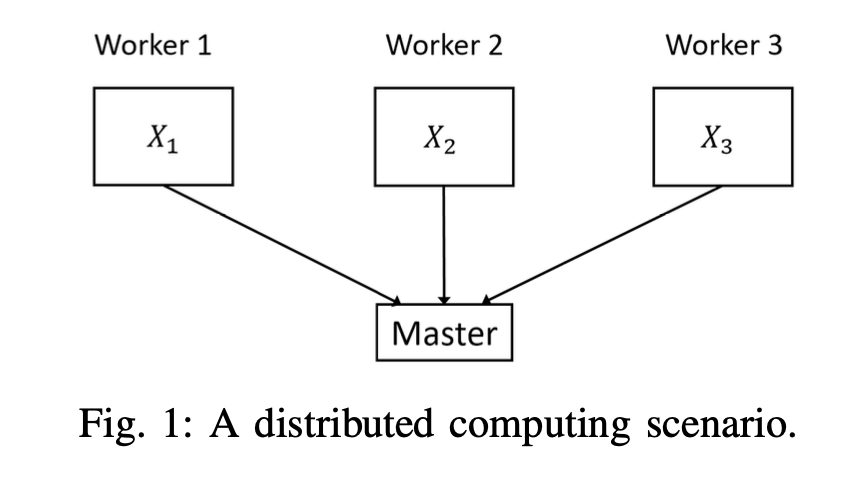
\includegraphics[keepaspectratio]{images/Fig-01.png}}
\caption{Descrption}
\end{figure}

    \begin{center}\rule{0.5\linewidth}{0.5pt}\end{center}

\paragraph{\texorpdfstring{\textbf{a) Distributing the
datasets}}{a) Distributing the datasets}}\label{a-distributing-the-datasets}

To ensure the master can recover all datasets \(W_1, W_2, W_3\) from
\textbf{any 2 workers}: 1. \textbf{Storage Capacity}: Each worker has a
storage capacity of \(200 \, \text{MB}\), and the total size of all
datasets is \(300 \, \text{MB}\). Therefore, each dataset must be
partially stored at multiple workers to enable recovery.

\begin{enumerate}
\def\labelenumi{\arabic{enumi}.}
\setcounter{enumi}{1}
\tightlist
\item
  \textbf{Data Distribution}:

  \begin{itemize}
  \tightlist
  \item
    Split each dataset \(W_1, W_2, W_3\) into \textbf{two equal parts}:
    \(W_{i,1}\) and \(W_{i,2}\) (e.g., \(W_1 = W_{1,1} + W_{1,2}\), each
    part \(50 \, \text{MB}\)).
  \item
    Assign the parts such that \textbf{any two workers have all parts of
    all datasets}. For instance:

    \begin{itemize}
    \tightlist
    \item
      Worker 1: \(W_{1,1}, W_{2,1}, W_{3,1}\) (150 MB total).
    \item
      Worker 2: \(W_{1,2}, W_{2,1}, W_{3,2}\) (150 MB total).
    \item
      Worker 3: \(W_{1,1}, W_{2,2}, W_{3,2}\) (150 MB total).
    \end{itemize}
  \end{itemize}

  This ensures that the master can recover \(W_1, W_2, W_3\) from any
  two workers since all parts of each dataset are distributed across at
  least two workers.
\end{enumerate}

\paragraph{\texorpdfstring{\textbf{b) Total rate \(R\) required (in
bits/ms)}}{b) Total rate R required (in bits/ms)}}\label{b-total-rate-r-required-in-bitsms}

\begin{itemize}
\item
  \textbf{Delay Constraint}: The master must recover all
  \(W_1, W_2, W_3\) (300 MB total) within \(10 \, \text{ms}\).
\item
  \textbf{Total Rate \(R\)}:
  \(R = \frac{\text{Total Size of Datasets (in bits)}}{\text{Delay Constraint (in ms)}}.\)

  \begin{itemize}
  \tightlist
  \item
    Total size of datasets =
    \(300 \, \text{MB} = 300 \times 8 \times 10^6 \, \text{bits} = 2.4 \times 10^9 \, \text{bits}\).
  \item
    Delay constraint = \(10 \, \text{ms} = 10^{-2} \, \text{s}\).
  \end{itemize}

  Substituting:
  \(R = \frac{2.4 \times 10^9}{10} = 2.4 \times 10^8 \, \text{bits/ms}.\)

  \textbf{Answer}: \(R = 240 \, \text{Mbps}\).
\end{itemize}

\paragraph{\texorpdfstring{\textbf{c) Total rate if the master can cache
one
dataset}}{c) Total rate if the master can cache one dataset}}\label{c-total-rate-if-the-master-can-cache-one-dataset}

\begin{itemize}
\item
  If the master caches one dataset, say \(W_1\), then it only needs to
  recover \(W_2\) and \(W_3\) from the workers.
\item
  Size of data to be transmitted:
  \(\text{Total Size} = W_2 + W_3 = 200 \, \text{MB} = 200 \times 8 \times 10^6 \, \text{bits} = 1.6 \times 10^9 \, \text{bits}.\)
\item
  \textbf{Total Rate \(R\)}:
  \(R = \frac{1.6 \times 10^9}{10} = 1.6 \times 10^8 \, \text{bits/ms}.\)

  \textbf{Answer}: \(R = 160 \, \text{Mbps}\).
\end{itemize}

\paragraph{\texorpdfstring{\textbf{d) Role of memory in transmission
rate}}{d) Role of memory in transmission rate}}\label{d-role-of-memory-in-transmission-rate}

\begin{itemize}
\tightlist
\item
  \textbf{Without Master Caching}: The master must recover all datasets
  (\(W_1, W_2, W_3\)) from the workers, resulting in a higher
  transmission rate (\(240 \, \text{Mbps}\)).
\item
  \textbf{With Master Caching}: The master pre-storing one dataset
  reduces the amount of data it needs to recover, thereby lowering the
  transmission rate (\(160 \, \text{Mbps}\)).
\end{itemize}

\textbf{Conclusion}: - Increasing the memory at the master node
significantly reduces the transmission rate required from the workers. -
Memory acts as a \textbf{trade-off between storage and communication
cost}, with more memory reducing the load on the communication channel.

    \(\color{orange}12\Bigl)\) \textbf{\emph{(1 point)}}. Name two
applications that in your opinion popularized Reinforcement Learning in
scientific communities working on Artificial Intelligence?

    \paragraph{\texorpdfstring{\textbf{Applications That Popularized
Reinforcement Learning
(RL):}}{Applications That Popularized Reinforcement Learning (RL):}}\label{applications-that-popularized-reinforcement-learning-rl}

\begin{enumerate}
\def\labelenumi{\arabic{enumi}.}
\tightlist
\item
  \textbf{Game Playing (e.g., AlphaGo, AlphaZero)}:

  \begin{itemize}
  \tightlist
  \item
    \textbf{Description}: RL gained significant attention with the
    development of DeepMind's \textbf{AlphaGo} and later
    \textbf{AlphaZero}, which used RL to achieve superhuman performance
    in complex games like Go, chess, and shogi.
  \item
    \textbf{Impact}: These breakthroughs demonstrated RL's capability to
    handle high-dimensional decision-making problems, inspiring its use
    in other domains.
  \end{itemize}
\item
  \textbf{Autonomous Robotics}:

  \begin{itemize}
  \tightlist
  \item
    \textbf{Description}: RL has been widely adopted in training robots
    to perform tasks such as walking, grasping, and manipulation. Robots
    learn optimal policies through interaction with their environments.
  \item
    \textbf{Impact}: Showcased RL's potential in real-world, dynamic,
    and uncertain environments, leading to advancements in robotics and
    control systems.
  \end{itemize}
\end{enumerate}

    \(\color{orange}13\Bigl)\) \textbf{\emph{(1 point)}}. AlphaZero is one
of the most exciting real-world applications that works using
Reinforcement Learning. Name the two algorithms that are used by
AlphaZero based on which this software achieves superior performance
compared to humans.

    The two key algorithms used by \textbf{AlphaZero} that enable its
superior performance are:

\begin{enumerate}
\def\labelenumi{\arabic{enumi}.}
\tightlist
\item
  \textbf{Monte Carlo Tree Search (MCTS)}:

  \begin{itemize}
  \tightlist
  \item
    \textbf{Description}: MCTS is a search algorithm used to explore
    possible moves in a game by simulating future outcomes and using the
    results to guide the search process.
  \item
    \textbf{Role in AlphaZero}: MCTS evaluates potential actions
    efficiently, focusing on the most promising moves, which helps
    AlphaZero make better decisions.
  \end{itemize}
\item
  \textbf{Deep Reinforcement Learning}:

  \begin{itemize}
  \tightlist
  \item
    \textbf{Description}: AlphaZero combines reinforcement learning with
    deep neural networks to approximate the value function (estimating
    the likelihood of winning) and the policy (deciding the best move).
  \item
    \textbf{Role in AlphaZero}: The neural network predicts move
    probabilities and board evaluations, guiding MCTS and improving its
    performance over time through self-play.
  \end{itemize}
\end{enumerate}

These two algorithms work together synergistically, with MCTS leveraging
the neural network's outputs and the network improving its predictions
through reinforcement learning.

    \(\color{orange}14\Bigl)\) \textbf{\emph{(1 point)}}. Name two classes
based on which one can distinguish exact dynamic programming algorithms?

    Two classes used to distinguish exact dynamic programming algorithms
are:

\begin{enumerate}
\def\labelenumi{\arabic{enumi}.}
\tightlist
\item
  \textbf{Value Iteration}:

  \begin{itemize}
  \tightlist
  \item
    Iteratively updates the value function for each state until
    convergence, focusing on finding the optimal value function.
  \end{itemize}
\item
  \textbf{Policy Iteration}:

  \begin{itemize}
  \tightlist
  \item
    Alternates between policy evaluation (calculating the value of a
    given policy) and policy improvement (updating the policy based on
    the value function) until an optimal policy is found.
  \end{itemize}
\end{enumerate}

    \(\color{orange}15\Bigl)\) \textbf{\emph{(1 point)}}. What is the
difference between deterministic and stochastic dynamic programming
algorithms?

    The key differences between \textbf{deterministic} and
\textbf{stochastic dynamic programming algorithms} are:

\begin{enumerate}
\def\labelenumi{\arabic{enumi}.}
\tightlist
\item
  \textbf{Nature of the Environment}:

  \begin{itemize}
  \tightlist
  \item
    \textbf{Deterministic}: Assumes the system evolves in a fully
    predictable manner, where the next state is uniquely determined by
    the current state and action.
  \item
    \textbf{Stochastic}: Accounts for uncertainty, where the next state
    depends on probabilistic transitions.
  \end{itemize}
\item
  \textbf{Transition Model}:

  \begin{itemize}
  \tightlist
  \item
    \textbf{Deterministic}: Uses fixed transition rules (e.g.,
    \(s_{t+1} = f(s_t, a_t)\)).
  \item
    \textbf{Stochastic}: Uses a probability distribution over possible
    transitions (e.g., \(P(s_{t+1} | s_t, a_t)\)).
  \end{itemize}
\item
  \textbf{Computation Complexity}:

  \begin{itemize}
  \tightlist
  \item
    \textbf{Deterministic}: Simpler and computationally less intensive
    due to the absence of randomness.
  \item
    \textbf{Stochastic}: More complex, as it requires handling
    probabilities and expectations over all possible transitions.
  \end{itemize}
\end{enumerate}

    \(\color{orange}16\Bigl)\) \textbf{\emph{(5 points)}}. Quantum. The two
components of the state
\(|\theta⟩= \frac{\sqrt(3)}{2\sqrt(2)}|11⟩+ \frac{\sqrt(5)}{2\sqrt(2)}|00⟩\)
are shared amidst Alice and Bob. In other words, Alice has the first
component and Bob has the second. Alice performs a measurement with two
outcomes \(\{{+1,−1}\}\). Outcome \(+1\) is associated with operator
\(|+⟩⟨+|\) and Outcome \(−1\) is associated with \(|−⟩⟨−|\). Bob
performs a measurement with two outcomes \(\{{+1,−1}\}\). Outcome \(+1\)
is associated with operator \(|0⟩⟨0|\) and Outcome \(−1\) is associated
with \(|1⟩⟨1|\).

\begin{enumerate}
\def\labelenumi{\alph{enumi})}
\item
  Before the measurement is performed, is the joint state entangled or
  separable?
\item
  Compute the probability of Alice observing \(-1\) and Bob observing
  \(+1\).
\item
  Compute the probability of Alice and Bob BOTH observing \(−1\).
\item
  Compute the probability of Alice and Bob BOTH observing \(+1\).
\item
  Identify the post measurement state when Alice observes \(+1\) and Bob
  observes \(−1\).
\end{enumerate}

    \begin{center}\rule{0.5\linewidth}{0.5pt}\end{center}

\paragraph{\texorpdfstring{\textbf{a) Is the joint state entangled or
separable?}}{a) Is the joint state entangled or separable?}}\label{a-is-the-joint-state-entangled-or-separable}

The state is:

\(|\theta\rangle = \frac{\sqrt{3}}{2\sqrt{2}} |11\rangle + \frac{\sqrt{5}}{2\sqrt{2}} |00\rangle.\)

\begin{itemize}
\tightlist
\item
  A state is \textbf{entangled} if it cannot be written as a tensor
  product of individual states,
  \(|\theta\rangle \neq |\phi_A\rangle \otimes |\phi_B\rangle\).
\item
  Here, \(|\theta\rangle\) is a superposition of \(|11\rangle\) and
  \(|00\rangle\), and it cannot be decomposed into separable parts for
  Alice and Bob.
\end{itemize}

\textbf{Answer}: The state is \textbf{entangled}.

\paragraph{\texorpdfstring{\textbf{b) Probability of Alice observing
\(-1\) and Bob observing
\(+1\):}}{b) Probability of Alice observing -1 and Bob observing +1:}}\label{b-probability-of-alice-observing--1-and-bob-observing-1}

\subparagraph{1. Measurement Operators:}\label{measurement-operators}

\begin{itemize}
\tightlist
\item
  Alice's measurement outcomes are:

  \begin{itemize}
  \tightlist
  \item
    \(+1\): \(|+\rangle = \frac{1}{\sqrt{2}}(|0\rangle + |1\rangle)\),
  \item
    \(-1\): \(|-\rangle = \frac{1}{\sqrt{2}}(|0\rangle - |1\rangle)\).
  \end{itemize}
\item
  Bob's measurement outcomes are:

  \begin{itemize}
  \tightlist
  \item
    \(+1\): \(|0\rangle\),
  \item
    \(-1\): \(|1\rangle\).
  \end{itemize}
\end{itemize}

\subparagraph{\texorpdfstring{2. Compute \(|\theta\rangle\) in the
measurement
basis:}{2. Compute \textbar\textbackslash theta\textbackslash rangle in the measurement basis:}}\label{compute-thetarangle-in-the-measurement-basis}

\(|\theta\rangle = \frac{\sqrt{3}}{2\sqrt{2}} |11\rangle + \frac{\sqrt{5}}{2\sqrt{2}} |00\rangle.\)

Express \(|1\rangle\) and \(|0\rangle\) in terms of \(|+\rangle\) and
\(|-\rangle\) for Alice:
\(|0\rangle = \frac{|+\rangle + |-\rangle}{\sqrt{2}}, \quad |1\rangle = \frac{|+\rangle - |-\rangle}{\sqrt{2}}.\)

Substituting for Alice's basis:
\(|11\rangle = \frac{1}{\sqrt{2}}(|+\rangle - |-\rangle)|1\rangle, \quad |00\rangle = \frac{1}{\sqrt{2}}(|+\rangle + |-\rangle)|0\rangle.\)

Expand:
\(|\theta\rangle = \frac{\sqrt{3}}{2\sqrt{2}} \cdot \frac{1}{\sqrt{2}} (|+\rangle - |-\rangle)|1\rangle + \frac{\sqrt{5}}{2\sqrt{2}} \cdot \frac{1}{\sqrt{2}} (|+\rangle + |-\rangle)|0\rangle.\)
\(|\theta\rangle = \frac{\sqrt{3}}{4} (|+\rangle - |-\rangle)|1\rangle + \frac{\sqrt{5}}{4} (|+\rangle + |-\rangle)|0\rangle.\)

\subparagraph{\texorpdfstring{3. Amplitude for \(|-\rangle|0\rangle\)
(Alice observes \(-1\), Bob observes
\(+1\)):}{3. Amplitude for \textbar-\textbackslash rangle\textbar0\textbackslash rangle (Alice observes -1, Bob observes +1):}}\label{amplitude-for--rangle0rangle-alice-observes--1-bob-observes-1}

The coefficient of \(|-\rangle|0\rangle\) is: \(\frac{\sqrt{5}}{4}.\)

\subparagraph{4. Probability:}\label{probability}

\(P(-1, +1) = \left|\frac{\sqrt{5}}{4}\right|^2 = \frac{5}{16}.\)

\paragraph{\texorpdfstring{\textbf{c) Probability of Alice and Bob BOTH
observing
\(-1\):}}{c) Probability of Alice and Bob BOTH observing -1:}}\label{c-probability-of-alice-and-bob-both-observing--1}

\subparagraph{\texorpdfstring{1. Amplitude for
\(|-\rangle|1\rangle\):}{1. Amplitude for \textbar-\textbackslash rangle\textbar1\textbackslash rangle:}}\label{amplitude-for--rangle1rangle}

The coefficient of \(|-\rangle|1\rangle\) is: \(-\frac{\sqrt{3}}{4}.\)

\subparagraph{2. Probability:}\label{probability-1}

\(P(-1, -1) = \left|-\frac{\sqrt{3}}{4}\right|^2 = \frac{3}{16}.\)

\paragraph{\texorpdfstring{\textbf{d) Probability of Alice and Bob BOTH
observing
\(+1\):}}{d) Probability of Alice and Bob BOTH observing +1:}}\label{d-probability-of-alice-and-bob-both-observing-1}

\subparagraph{\texorpdfstring{1. Amplitude for
\(|+\rangle|0\rangle\):}{1. Amplitude for \textbar+\textbackslash rangle\textbar0\textbackslash rangle:}}\label{amplitude-for-rangle0rangle}

The coefficient of \(|+\rangle|0\rangle\) is: \(\frac{\sqrt{5}}{4}.\)

\subparagraph{2. Probability:}\label{probability-2}

\(P(+1, +1) = \left|\frac{\sqrt{5}}{4}\right|^2 = \frac{5}{16}.\)

\paragraph{\texorpdfstring{\textbf{e) Post-measurement state when Alice
observes \(+1\) and Bob observes
\(-1\):}}{e) Post-measurement state when Alice observes +1 and Bob observes -1:}}\label{e-post-measurement-state-when-alice-observes-1-and-bob-observes--1}

\subparagraph{1. Projection:}\label{projection}

The projection operator for this outcome is:
\(P_{+1, -1} = (|+\rangle \langle +|) \otimes (|1\rangle \langle 1|).\)

Apply this to \(|\theta\rangle\):
\(|\theta'\rangle = P_{+1, -1} |\theta\rangle.\)

From the expanded \(|\theta\rangle\), the term contributing to
\(|+\rangle|1\rangle\) has coefficient: \(\frac{\sqrt{3}}{4}.\)

\subparagraph{2. Normalize:}\label{normalize}

\(|\theta'\rangle = \frac{|+\rangle|1\rangle}{\sqrt{P(+1, -1)}}.\)

Probability \(P(+1, -1)\):
\(P(+1, -1) = \left|\frac{\sqrt{3}}{4}\right|^2 = \frac{3}{16}.\)

Normalized state:
\(|\theta'\rangle = \frac{|+\rangle|1\rangle}{\sqrt{\frac{3}{16}}} = \frac{4}{\sqrt{3}} |+\rangle|1\rangle.\)

\paragraph{\texorpdfstring{\textbf{Summary of
Answers:}}{Summary of Answers:}}\label{summary-of-answers}

\begin{enumerate}
\def\labelenumi{\alph{enumi})}
\tightlist
\item
  The state is \textbf{entangled}.\\
\item
  \(P(-1, +1) = \frac{5}{16}\).\\
\item
  \(P(-1, -1) = \frac{3}{16}\).\\
\item
  \(P(+1, +1) = \frac{5}{16}\).\\
\item
  Post-measurement state:
  \(|\theta'\rangle = \frac{4}{\sqrt{3}} |+\rangle|1\rangle\).
\end{enumerate}

    \begin{tcolorbox}[breakable, size=fbox, boxrule=1pt, pad at break*=1mm,colback=cellbackground, colframe=cellborder]
\prompt{In}{incolor}{ }{\boxspacing}
\begin{Verbatim}[commandchars=\\\{\}]

\end{Verbatim}
\end{tcolorbox}


    % Add a bibliography block to the postdoc
    
    
    
\end{document}
